% Provenance (never printed): cycle 3 / 6e "La planete Terre, l'environnement
% et l'action humaine" (the Earth in the Solar System; conditions for life);
% see sources/book1/PROVENANCE.md. Book 1, grade 6, chapter 1.
\chapter{De Aarde, een planeet van het zonnestelsel}\label{ch:g6:earth-a-planet}

Er zijn drie robotsondes de ruimte in gestuurd. Een voor een sturen ze een
foto naar huis, als een ansichtkaart. De eerste komt van Venus: een bleke
bol, gehuld in dikke \omterm{def:g4:clouds-rain-snow:cloud}{wolken}, waar het heet genoeg is om lood te smelten en
de lucht met een verpletterend gewicht op de grond drukt. De tweede komt
van Mars: een rode, koude, stoffige \omterm{def:g5:weather-and-climate:desert}{woestijn} onder een ijle hemel. De derde
sonde heeft haar camera teruggedraaid naar huis: een blauw-witte bol, met
\omterm{def:g2:water-on-earth:ocean}{oceanen}, \omterm{def:g4:clouds-rain-snow:cloud}{wolken} en ijs. Drie planeten, buren rond dezelfde Zon. Waarom is
er maar één blauw?
% ledger: nasa:venus-clouds, nasa:mars-water

\begin{omfigure}
\begin{minipage}[t]{0.31\linewidth}\centering
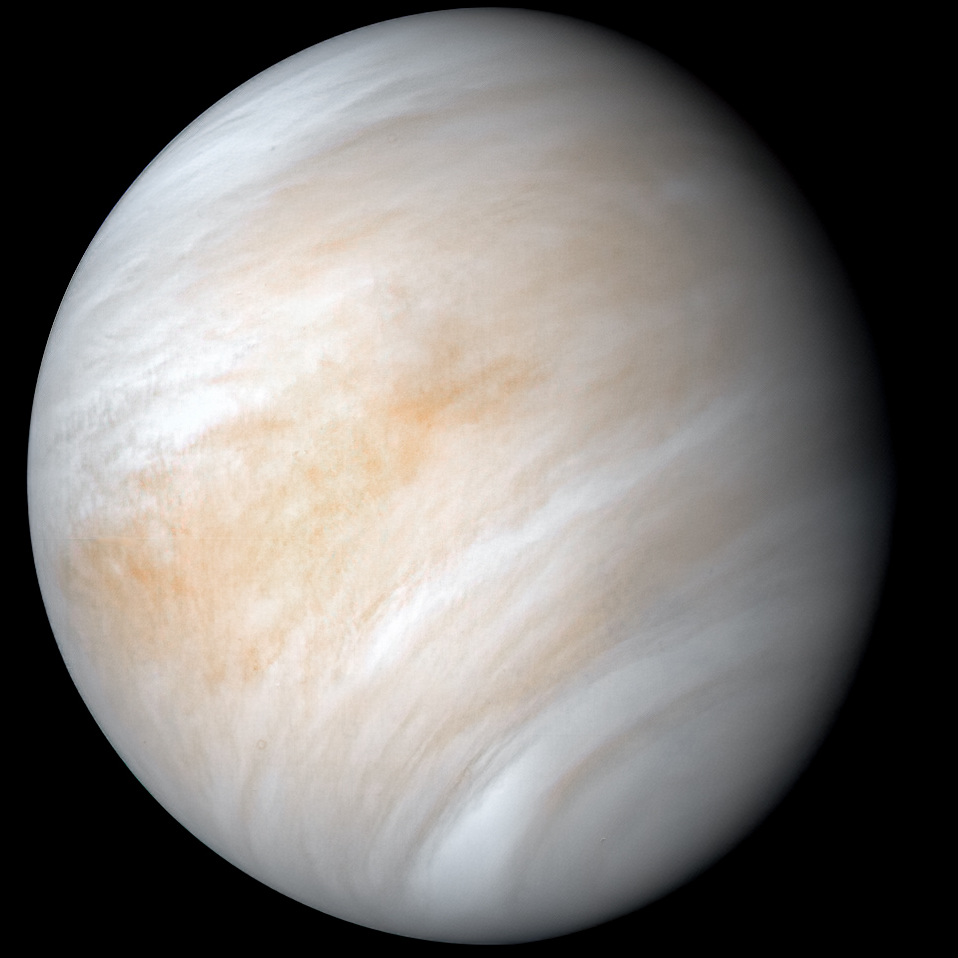
\includegraphics[width=\linewidth]{images/book1/g6-venus-mariner10.jpg}\\[2pt]
{\small Venus}
\end{minipage}\hfill
\begin{minipage}[t]{0.31\linewidth}\centering
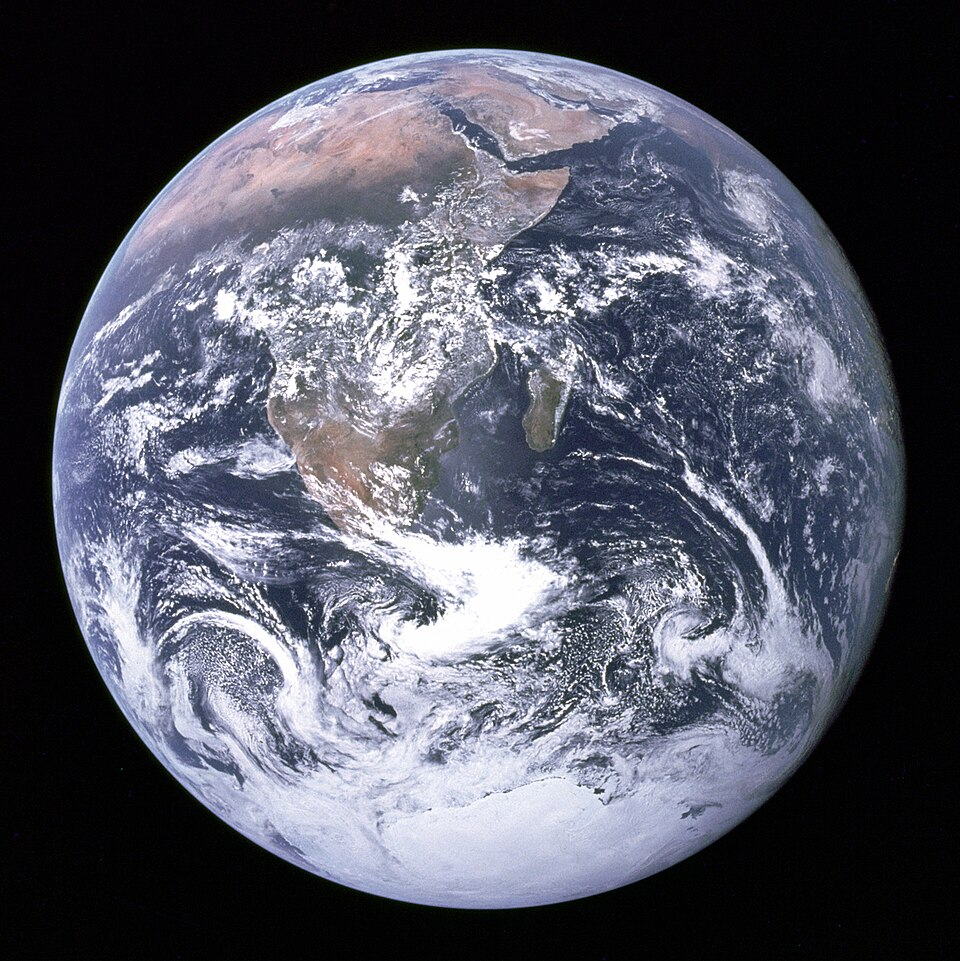
\includegraphics[width=\linewidth]{images/book1/g6-earth-apollo17.jpg}\\[2pt]
{\small De Aarde}
\end{minipage}\hfill
\begin{minipage}[t]{0.31\linewidth}\centering
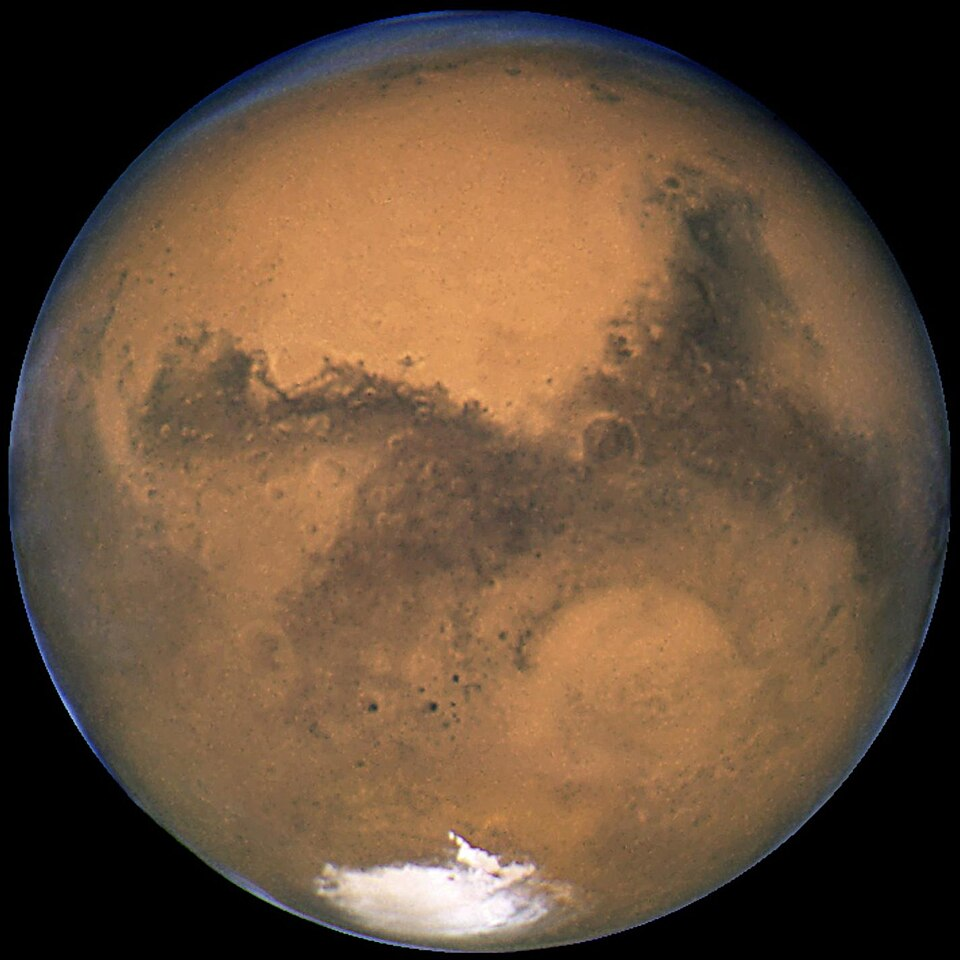
\includegraphics[width=\linewidth]{images/book1/g6-mars-hubble.jpg}\\[2pt]
{\small Mars}
\end{minipage}

\medskip
{\small Drie ansichtkaarten uit de ruimte. Venus, gefotografeerd door de
sonde Mariner~10 in 1974: we zien alleen de bovenkant van haar \omterm{def:g4:clouds-rain-snow:cloud}{wolken}. De
Aarde, gefotografeerd door de bemanning van Apollo~17 op weg naar de Maan
in 1972: Afrika, Arabië en het ijs van Antarctica onder witte \omterm{def:g4:clouds-rain-snow:cloud}{wolken}. Mars,
gefotografeerd door de Hubble-ruimtetelescoop in 2003, met een witte kap
van ijs op zijn \omterm{def:g3:continents-and-oceans:poles}{pool}. (Foto's: NASA/JPL-Caltech; NASA; NASA, ESA en het
Hubble Heritage Team.)}
% ledger: nasa:venus-mariner10, nasa:apollo17-earth, hubble:mars-2003
\end{omfigure}

\begin{recall}
De natuurkundeboeken lieten zien dat de Zon een ster is, een enorme bol
heet gas die uit zichzelf licht geeft, en dat een planeet een groot, rond
hemellichaam is dat om een ster draait en zelf geen licht geeft: we zien
het omdat het het licht van zijn ster terugkaatst. De Zon en alles wat om
haar heen draait, vormen het zonnestelsel. Elke planeet beweegt om de Zon
langs een baan, en draait om zichzelf rond een as. De lucht om ons heen
drukt op alles wat ze raakt: dat is de luchtdruk. De dichtheid van een
stof zegt hoe zwaar een bepaald volume ervan is: één kubieke centimeter
water weegt 1~gram, dus zijn dichtheid is 1~gram per kubieke centimeter;
een stof met een grotere dichtheid dan water zinkt erin, een stof met een
kleinere dichtheid drijft. Ten slotte is ongeveer zeven tiende van het
aardoppervlak bedekt door de \omterm{def:g2:water-on-earth:ocean}{oceaan} (\cref{ch:g2:water-on-earth}).
\end{recall}

\section{Acht planeten rond de Zon}

Acht planeten bewegen rond de Zon. Op volgorde, van de dichtstbijzijnde
tot de verste, zijn dat Mercurius, Venus, de Aarde, Mars, Jupiter,
Saturnus, Uranus en Neptunus. Een zinnetje kan helpen om de volgorde te
onthouden: \emph{Mijn Vader At Mosselen, Jij Smulde Uren Na} (Mercurius,
Venus, Aarde, Mars, Jupiter, Saturnus, Uranus, Neptunus).

De tekening hieronder laat de acht planeten naast elkaar zien, op dezelfde
schaal getekend: als een planeet twee keer zo breed is als een andere, is
haar cirkel ook twee keer zo breed.

\begin{omfigure}
\pgfplotstableread{figdata/out/grade-6-planets-sizes.dat}\gsixsizes
\begin{tikzpicture}
  \draw[black!40] (-0.2,0) -- (13.8,0);
  \pgfplotstablegetrowsof{\gsixsizes}
  \pgfmathtruncatemacro{\gsixlast}{\pgfplotsretval-1}
  \foreach \i in {0,...,\gsixlast}{
    \pgfplotstablegetelem{\i}{x_cm}\of\gsixsizes \let\gx\pgfplotsretval
    \pgfplotstablegetelem{\i}{d_cm}\of\gsixsizes \let\gd\pgfplotsretval
    \edef\gn{\ifcase\i\space Mercurius\or Venus\or Aarde\or Mars\or Jupiter\or Saturnus\or Uranus\or Neptunus\fi}
    \pgfplotstablegetelem{\i}{d_km}\of\gsixsizes \let\gk\pgfplotsretval
    \pgfmathsetmacro{\gr}{\gd/2}
    \ifnum\i<4
      \fill[brown!70!black, draw=black!60, line width=0.3pt] (\gx,\gr) circle (\gr);
    \else
      \fill[orange!35, draw=black!60, line width=0.3pt] (\gx,\gr) circle (\gr);
    \fi
    \node[font=\scriptsize, rotate=40, anchor=north east, inner sep=1pt]
      at (\gx+0.08,-0.08) {\gn};
  }
  \node[font=\scriptsize, align=left, anchor=north west] at (-0.2,4.15)
    {\tikz\fill[brown!70!black, draw=black!60] (0,0) circle (2.2pt); rotsplaneten\\
     \tikz\fill[orange!35, draw=black!60] (0,0) circle (2.2pt); reuzenplaneten};
  \draw[|-|, black!70] (0,2.2) -- (1,2.2)
    node[midway, above, font=\scriptsize] {35\,000 km};
\end{tikzpicture}

{\small De acht planeten op schaal getekend (diameters uit het planetaire
overzicht van NASA). De afstanden tussen de planeten zijn niet op schaal:
die zijn veel te groot om op een bladzijde te passen.}
% ledger: planet:Mercury.diameter, planet:Venus.diameter, planet:Earth.diameter, planet:Mars.diameter, planet:Jupiter.diameter, planet:Saturn.diameter, planet:Uranus.diameter, planet:Neptune.diameter (figdata/grade-6/planets.py, part sizes)
\end{omfigure}

De vier planeten die het dichtst bij de Zon staan, zijn klein. De volgende
vier zijn reuzen: Jupiter is ongeveer 11 keer zo breed als de Aarde. En de
Zon? Op dezelfde schaal getekend als de planeten hierboven zou ze een
schijf van ongeveer 40~centimeter doorsnede zijn --- breder dan deze
bladzijde.
% ledger: planet:Jupiter.diameter, planet:Earth.diameter, sun:R (planets.py: sun_cm = 39.9 cm)

Grootte is niet het enige verschil. De tabel hieronder geeft voor elke
planeet de diameter, de dichtheid (in gram per kubieke centimeter) en de
afstand tot de Zon.

\begin{center}
\small
\begin{tabular}{lrrrr}
\hline
planeet & diameter (km) & dichtheid (g/cm$^3$) & afstand tot de Zon (miljoen km)\\
\hline
Mercurius & 4\,879 & 5.4 & 58\\
Venus & 12\,104 & 5.2 & 108\\
Aarde & 12\,756 & 5.5 & 150\\
Mars & 6\,792 & 3.9 & 228\\
\hline
Jupiter & 142\,984 & 1.3 & 779\\
Saturnus & 120\,536 & 0.7 & 1\,432\\
Uranus & 51\,118 & 1.3 & 2\,867\\
Neptunus & 49\,528 & 1.6 & 4\,515\\
\hline
\end{tabular}
% ledger: planet:Mercury.diameter, planet:Venus.diameter, planet:Earth.diameter, planet:Mars.diameter, planet:Jupiter.diameter, planet:Saturn.diameter, planet:Uranus.diameter, planet:Neptune.diameter, planet:Mercury.density, planet:Venus.density, planet:Earth.density, planet:Mars.density, planet:Jupiter.density, planet:Saturn.density, planet:Uranus.density, planet:Neptune.density, planet:Mercury.dist, planet:Venus.dist, planet:Earth.dist, planet:Mars.dist, planet:Jupiter.dist, planet:Saturn.dist, planet:Uranus.dist, planet:Neptune.dist (figdata/grade-6/planets.py, main table)
\end{center}

De dichtheden verdelen de planeten in twee families, zonder iets ertussen:
de eerste vier zijn dicht, meer dan 3.9~gram per kubieke centimeter, zoals
\omterm{def:g3:stones-pebbles-sand:rock}{gesteente} en metaal; de laatste vier zijn licht, minder dan 1.7~gram per
kubieke centimeter.

\begin{definition}[Rotsplaneten en reuzenplaneten]\label{def:g6:earth-a-planet:planet-types}
Een \emph{rotsplaneet}\index{rotsplaneet} is een kleine planeet met een
grote dichtheid, gemaakt van \omterm{def:g3:stones-pebbles-sand:rock}{gesteente} en metaal, met een vast oppervlak
waarop een sonde kan landen: Mercurius, Venus, de Aarde en Mars. Een
\emph{reuzenplaneet}\index{reuzenplaneet} is een heel grote planeet met een
kleine dichtheid, die vooral bestaat uit gassen en vloeistoffen, zonder
vast oppervlak om op te landen: Jupiter, Saturnus, Uranus en Neptunus.
% ledger: nasa:planet-families
\end{definition}

\begin{omfigure}
\begin{minipage}[c]{0.6\linewidth}\centering
\begin{tikzpicture}
  \begin{axis}[ybar, bar width=11pt, width=\linewidth, height=5.4cm,
      ymin=0, ymax=6.2, xmin=-0.6, xmax=7.6,
      xtick={0,...,7}, xticklabels={Mercurius,Venus,Aarde,Mars,Jupiter,Saturnus,Uranus,Neptunus},
      xticklabel style={rotate=40, anchor=north east, font=\scriptsize},
      ytick={0,1,...,6}, ylabel={dichtheid (g/cm$^3$)},
      tick label style={font=\scriptsize}, label style={font=\scriptsize},
      axis x line*=bottom, axis y line*=left]
    \addplot[fill=brown!70!black, draw=black!60, bar shift=0pt, restrict x to domain=0:3]
      table[x=idx, y=density_gcm3] {figdata/out/grade-6-planets-density.dat};
    \addplot[fill=orange!35, draw=black!60, bar shift=0pt, restrict x to domain=4:7]
      table[x=idx, y=density_gcm3] {figdata/out/grade-6-planets-density.dat};
    \draw[blue!60!black, densely dashed] (axis cs:-0.6,1) -- (axis cs:7.6,1);
    \node[font=\scriptsize, blue!60!black, anchor=south, inner sep=1pt]
      at (axis cs:5,1) {water};
  \end{axis}
\end{tikzpicture}
\end{minipage}\hfill
\begin{minipage}[c]{0.36\linewidth}\centering
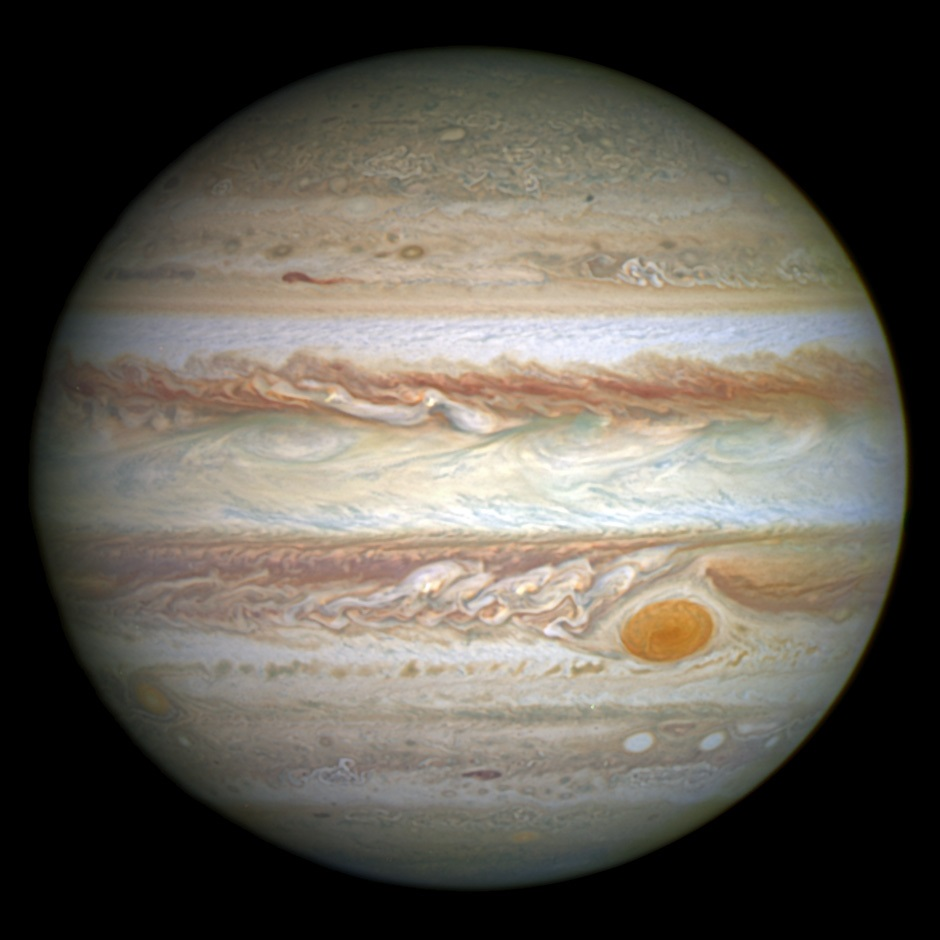
\includegraphics[width=0.9\linewidth]{images/book1/g6-jupiter-hubble.jpg}\\[2pt]
{\small Jupiter, gefotografeerd door de Hubble-ruimtetelescoop in 2014.
(Foto: NASA, ESA, A.~Simon.)}
% ledger: hubble:jupiter-2014
\end{minipage}

\smallskip
{\small Links: de dichtheid van de acht planeten; de stippellijn is de
dichtheid van water. Rechts: wat we van een \omterm{def:g6:earth-a-planet:planet-types}{reuzenplaneet} zien, is de
bovenkant van haar \omterm{def:g4:clouds-rain-snow:cloud}{wolken}.}
% ledger: planet:Mercury.density, planet:Venus.density, planet:Earth.density, planet:Mars.density, planet:Jupiter.density, planet:Saturn.density, planet:Uranus.density, planet:Neptune.density (figdata/grade-6/planets.py, part density)
\end{omfigure}

De foto van Jupiter laat banden van \omterm{def:g4:clouds-rain-snow:cloud}{wolken} zien, licht en donker, en een
rode ovaal: de Grote Rode Vlek, een reusachtige \omterm{def:g5:natural-hazards:storm}{storm} groter dan de hele
Aarde, die al honderden jaren raast. Onder de \omterm{def:g4:clouds-rain-snow:cloud}{wolken} is er geen grond:
alleen gassen, vooral waterstof en helium, die steeds dichter worden naarmate
je dieper gaat.
% ledger: nasa:jupiter-gas

\begin{remark}[Een planeet lichter dan water]\label{rem:g6:earth-a-planet:saturn}
Saturnus is de enige planeet met een kleinere dichtheid dan water:
ongeveer 0.7~gram per kubieke centimeter. Als er een badkuip bestond die
groot genoeg was om hem te bevatten, zou Saturnus blijven drijven!
% ledger: nasa:saturn-float, planet:Saturn.density
\end{remark}

\section{Hoe ver liggen de planeten uit elkaar?}

De planeten verschillen niet alleen sterk in grootte; ze staan ook heel ver
van elkaar af. De Aarde staat ongeveer 150~miljoen kilometer van de Zon.
Neptunus, de verste planeet, staat 30~keer zo ver: ongeveer 4500~miljoen
kilometer. De tekening hieronder zet de acht planeten op één lijn, op hun
afstanden tot de Zon, op schaal.
% ledger: planet:Earth.dist, planet:Neptune.dist

\begin{omfigure}
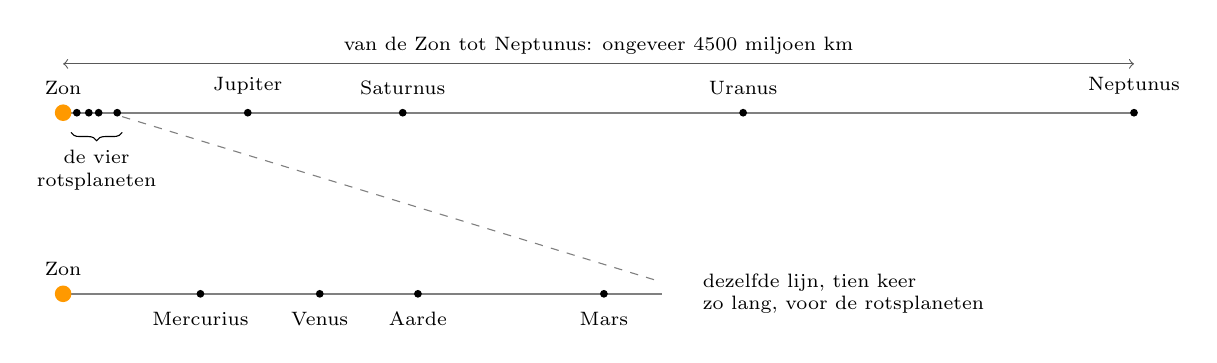
\begin{tikzpicture}
  % whole system
  \draw[thick, gray] (0,0) -- (13.6,0);
  \fill[orange!80!yellow] (0,0) circle (3pt);
  \node[font=\scriptsize, above=3pt] at (0,0) {Zon};
  \foreach \n/\x/\lab in {Mercury/0.174/, Venus/0.326/, Earth/0.451/, Mars/0.687/,
                          Jupiter/2.345/Jupiter, Saturn/4.313/Saturnus, Uranus/8.636/Uranus, Neptune/13.6/Neptunus} {
    \fill (\x,0) circle (1.4pt);
    \node[font=\scriptsize, above=3pt] at (\x,0) {\lab};
  }
  \draw[decorate, decoration={brace, amplitude=3pt, mirror}] (0.1,-0.25) -- (0.75,-0.25)
    node[midway, below=3pt, font=\scriptsize, align=center] {de vier\\ rotsplaneten};
  \draw[<->, thin, gray!70!black] (0,0.62) -- (13.6,0.62) node[midway, above, font=\scriptsize, black] {van de Zon tot Neptunus: ongeveer 4500 miljoen km};
  % the inner system, ten times larger
  \begin{scope}[yshift=-2.3cm]
    \draw[thick, gray] (0,0) -- (7.6,0);
    \fill[orange!80!yellow] (0,0) circle (3pt);
    \node[font=\scriptsize, above=3pt] at (0,0) {Zon};
    \foreach \n/\x in {Mercurius/1.744, Venus/3.259, Aarde/4.506, Mars/6.868} {
      \fill (\x,0) circle (1.4pt);
      \node[font=\scriptsize, below=3pt] at (\x,0) {\n};
    }
    \node[font=\scriptsize, anchor=west, align=left] at (8.0,0) {dezelfde lijn, tien keer\\ zo lang, voor de rotsplaneten};
  \end{scope}
  \draw[dashed, gray] (0.75,-0.05) -- (7.6,-2.15);
\end{tikzpicture}

{\small De afstanden van de planeten tot de Zon, op schaal. Boven: het hele
zonnestelsel, van de Zon tot Neptunus. Onder: de vier \omterm{def:g6:earth-a-planet:planet-types}{rotsplaneten}, tien
keer vergroot. De grootte van de stippen is niet op schaal.}
% ledger: planet:Mercury.dist, planet:Venus.dist, planet:Earth.dist, planet:Mars.dist, planet:Jupiter.dist, planet:Saturn.dist, planet:Uranus.dist, planet:Neptune.dist (figdata/grade-6/planets.py, part dist)
\end{omfigure}

De vier \omterm{def:g6:earth-a-planet:planet-types}{rotsplaneten} staan allemaal dicht bij de Zon; de vier
\omterm{def:g6:earth-a-planet:planet-types}{reuzenplaneten} staan ver weg, met enorme afstanden ertussen. Alleen al de afstand tussen Mars en Jupiter, ongeveer 550~miljoen kilometer, is meer dan twee keer de afstand van de Zon tot Mars.
% ledger: planet:Mars.dist, planet:Jupiter.dist

Het is moeilijk om groottes en afstanden op dezelfde schaal te tekenen: de
planeten worden onzichtbare stipjes. Een \emph{schaalmodel} helpt om je
allebei tegelijk voor te stellen.

\begin{method}[Een schaalmodel van het zonnestelsel bouwen]\label{met:g6:earth-a-planet:scale-model}
\begin{enumerate}
  \item Kies de grootte van de Aarde in het model, bijvoorbeeld 1~cm.
  \item Zoek uit voor hoeveel echte kilometer 1~cm in het model staat: deel
        de echte diameter van de Aarde (12\,756~km) door haar grootte in het
        model.
  \item Deel elke echte grootte en elke echte afstand door dit getal.
        Zet daarna de eenheden om in iets wat je je makkelijk kunt
        voorstellen (centimeter, meter, kilometer).
\end{enumerate}
% ledger: planet:Earth.diameter
\end{method}

\begin{example}[Een knikker als Aarde]\label{ex:g6:earth-a-planet:marble}
Als de Aarde een knikker van 1~cm breed is, staat 1~cm voor 12\,756~km. De
Zon, met een doorsnede van 1\,391\,400~km, wordt een bal van $1\,391\,400 \div 12\,756 \approx
109$~cm breed: een bal groter dan een klein kind. De Aarde staat 150~miljoen~km van de Zon:
$149\,600\,000 \div 12\,756 \approx 11\,700$~cm, dat is ongeveer 117~meter,
de lengte van een voetbalveld.
% ledger: planet:Earth.diameter, sun:R, planet:Earth.dist
\end{example}

\begin{center}\small
\begin{tabular}{|l|c|c|}
\hline
\textbf{hemellichaam} & \textbf{grootte in het model (cm)} & \textbf{afstand tot de Zon (m)} \\
\hline
de Zon & 109 & --- \\
Mercurius & 0.38 & 45 \\
Venus & 0.95 & 85 \\
de Aarde & 1.00 & 117 \\
Mars & 0.53 & 179 \\
Jupiter & 11.21 & 610 \\
Saturnus & 9.45 & 1123 \\
Uranus & 4.01 & 2248 \\
Neptunus & 3.88 & 3540 \\
\hline
\end{tabular}
\end{center}
% ledger: sun:R, planet:Mercury.diameter, planet:Venus.diameter, planet:Earth.diameter, planet:Mars.diameter, planet:Jupiter.diameter, planet:Saturn.diameter, planet:Uranus.diameter, planet:Neptune.diameter, planet:Mercury.dist, planet:Venus.dist, planet:Earth.dist, planet:Mars.dist, planet:Jupiter.dist, planet:Saturn.dist, planet:Uranus.dist, planet:Neptune.dist (figdata/grade-6/planets.py, part model)

In dit model beslaat het hele zonnestelsel tot en met Neptunus een cirkel
van 7~km doorsnede, met een grote bal in het midden en acht knikkers en
ballen, de grootste zo groot als een grapefruit, daaroverheen verspreid. Het
zonnestelsel is grotendeels lege ruimte.

\section{Venus, de Aarde en Mars}

Venus, de Aarde en Mars zijn buren, alle drie \omterm{def:g6:earth-a-planet:planet-types}{rotsplaneten}. Venus is
bijna even groot als de Aarde: haar diameter is 95~\% van die van de
Aarde. Mars is kleiner: zijn diameter is ongeveer de helft van die van de
Aarde. Toch kunnen deze drie planeten bijna niet meer van elkaar
verschillen.
% ledger: planet:Venus.diameter, planet:Earth.diameter, planet:Mars.diameter (planets.py: 94.9 %)

\paragraph{Venus.} Venus is gehuld in een dikke laag lucht, die vooral uit
koolstofdioxide bestaat, met dichte \omterm{def:g4:clouds-rain-snow:cloud}{wolken} van zwavelzuur, een bijtend
zuur. Haar lucht is zo dik dat ze 92~keer zo hard op de grond drukt als de
lucht van de Aarde op die van ons. Aan het oppervlak is de temperatuur
ongeveer 464~$^\circ$C: heet genoeg om lood te smelten. Daar kan geen
water vloeibaar blijven.
% ledger: nasa:venus-clouds, planet:Venus.psurf, planet:Venus.Tmean

\paragraph{Mars.} Mars is een koude, droge, stoffige \omterm{def:g5:weather-and-climate:desert}{woestijn}. Zijn lucht
bestaat ook vooral uit koolstofdioxide, maar is heel ijl: ze drukt ongeveer
honderd keer minder op de grond dan de lucht van de Aarde. De gemiddelde
temperatuur is $-65$~$^\circ$C. Er is nu water op Mars, maar bevroren: als
ijs in de poolkappen en onder de grond bij de \omterm{def:g3:continents-and-oceans:poles}{polen}. Toch is Mars niet
altijd zo geweest: miljarden jaren geleden stroomden er \omterm{def:g1:landscapes-around-us:water}{rivieren} op Mars,
ontstonden er \omterm{def:g1:landscapes-around-us:water}{meren} en trokken er \omterm{def:g5:water-shapes-the-land:flood}{overstromingen} overheen.
% ledger: nasa:mars-water, planet:Mars.psurf, planet:Mars.Tmean

\paragraph{De Aarde.} Tussen die twee in heeft de Aarde lucht die met
ongeveer 1~bar op de grond drukt (de eenheid waarmee we de luchtdruk op de
planeten vergelijken), een gemiddelde temperatuur van 15~$^\circ$C, en
\omterm{def:g2:water-on-earth:ocean}{oceanen} van vloeibaar water.
% ledger: planet:Earth.psurf, planet:Earth.Tmean

\begin{omfigure}
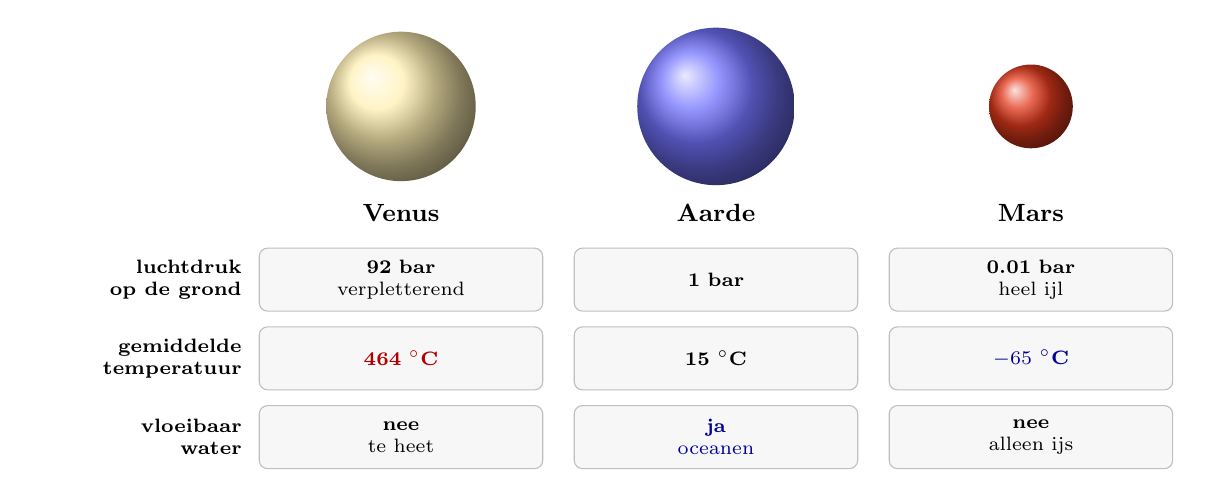
\begin{tikzpicture}[x=1cm, y=1cm,
    lab/.style={font=\scriptsize, align=center, text width=3.6cm},
    row/.style={font=\scriptsize\bfseries, anchor=east, align=right, text width=2.6cm}]
  % discs to scale: diameters 94.9 %, 100 %, 53.2 % of the Earth's (planets.py)
  \shade[ball color=yellow!60!orange!30] (3,0) circle (0.949);
  \shade[ball color=blue!55] (7,0) circle (1.0);
  \shade[ball color=red!55!brown] (11,0) circle (0.532);
  \node[font=\small\bfseries] at (3,-1.35) {Venus};
  \node[font=\small\bfseries] at (7,-1.35) {Aarde};
  \node[font=\small\bfseries] at (11,-1.35) {Mars};
  \foreach \y/\t in {-2.2/{luchtdruk\\op de grond}, -3.2/{gemiddelde\\temperatuur},
                     -4.2/{vloeibaar\\water}}
    {\node[row] at (1.1,\y) {\t};}
  \foreach \x in {3,7,11}{
    \foreach \y in {-2.2,-3.2,-4.2}{
      \draw[rounded corners=3pt, black!25, fill=black!3] (\x-1.8,\y-0.4) rectangle (\x+1.8,\y+0.4);}}
  \node[lab] at (3,-2.2) {\textbf{92 bar}\\verpletterend};
  \node[lab] at (7,-2.2) {\textbf{1 bar}};
  \node[lab] at (11,-2.2) {\textbf{0.01 bar}\\heel ijl};
  \node[lab, text=red!70!black] at (3,-3.2) {\textbf{464~$^\circ$C}};
  \node[lab] at (7,-3.2) {\textbf{15~$^\circ$C}};
  \node[lab, text=blue!60!black] at (11,-3.2) {\textbf{$-65$~$^\circ$C}};
  \node[lab] at (3,-4.2) {\textbf{nee}\\te heet};
  \node[lab, text=blue!60!black] at (7,-4.2) {\textbf{ja}\\oceanen};
  \node[lab] at (11,-4.2) {\textbf{nee}\\alleen ijs};
\end{tikzpicture}

{\small Venus, de Aarde en Mars vergeleken. De drie schijven zijn op schaal
getekend. (Waarden: planetair overzicht van NASA.)}
% ledger: planet:Venus.psurf, planet:Earth.psurf, planet:Mars.psurf, planet:Mercury.Tmean, planet:Venus.Tmean, planet:Earth.Tmean, planet:Mars.Tmean, planet:Jupiter.Tmean, planet:Saturn.Tmean, planet:Uranus.Tmean, planet:Neptune.Tmean, nasa:mars-water
\end{omfigure}

\paragraph{Heet en koud.} Dicht bij de Zon krijgt een planeet veel van haar
licht en warmte; ver weg heel weinig. Hoe verder een planeet van de Zon
staat, hoe kouder ze dus zou moeten zijn. Het diagram hieronder laat zien
dat dit klopt vanaf de Aarde naar buiten: de \omterm{def:g6:earth-a-planet:planet-types}{reuzenplaneten}, ver weg, zijn
bevroren werelden. Maar kijk naar Venus: ze staat bijna twee keer zo ver
van de Zon als Mercurius, en toch is ze heter! Haar dikke lucht van
koolstofdioxide houdt de warmte van de Zon vast als een zware deken en
laat haar niet ontsnappen. Mercurius, met bijna geen lucht, kan zijn
warmte niet vasthouden.
% ledger: planet:Mercury.Tmean, planet:Venus.Tmean, planet:Earth.Tmean, planet:Mars.Tmean, planet:Jupiter.Tmean, planet:Saturn.Tmean, planet:Uranus.Tmean, planet:Neptune.Tmean, planet:Mercury.dist, planet:Venus.dist, planet:Earth.dist, planet:Mars.dist, planet:Jupiter.dist, planet:Saturn.dist, planet:Uranus.dist, planet:Neptune.dist, nasa:venus-clouds, planet:Mercury.psurf

\begin{omfigure}
\begin{tikzpicture}
  \begin{axis}[ybar, bar width=14pt, width=0.86\linewidth, height=6cm,
      ymin=-270, ymax=520, xmin=-0.6, xmax=7.6,
      xtick={0,...,7},
      xticklabels={{Mercurius\\58}, {Venus\\108}, {Aarde\\150}, {Mars\\228},
                   {Jupiter\\779}, {Saturnus\\1432}, {Uranus\\2867}, {Neptunus\\4515}},
      xticklabel style={align=center, font=\scriptsize},
      axis x line*=bottom, axis y line*=left,
      xticklabel pos=lower, ytick={-200,-100,...,500},
      ylabel={gemiddelde temperatuur ($^\circ$C)}, xlabel={planeet en afstand tot de Zon (miljoen km)},
      tick label style={font=\scriptsize}, label style={font=\scriptsize},
      nodes near coords, nodes near coords style={font=\tiny},
      every node near coord/.append style={/pgf/number format/1000 sep={}}]
    \addplot[fill=orange!50, draw=black!60, bar shift=0pt]
      table[x=idx, y=tmean_C] {figdata/out/grade-6-planets-temp.dat};
    \draw[black!50] (axis cs:-0.6,0) -- (axis cs:7.6,0);
  \end{axis}
\end{tikzpicture}

{\small De gemiddelde temperatuur van de planeten, op volgorde van afstand
tot de Zon. Venus breekt de regel: ze is heter dan Mercurius, die dichter
bij de Zon staat. (Waarden: planetair overzicht van NASA.)}
% ledger: planet:Mercury.Tmean, planet:Venus.Tmean, planet:Earth.Tmean, planet:Mars.Tmean, planet:Jupiter.Tmean, planet:Saturn.Tmean, planet:Uranus.Tmean, planet:Neptune.Tmean, planet:Mercury.dist, planet:Venus.dist, planet:Earth.dist, planet:Mars.dist, planet:Jupiter.dist, planet:Saturn.dist, planet:Uranus.dist, planet:Neptune.dist (figdata/grade-6/planets.py, part temp)
\end{omfigure}

\section{Wat leven op Aarde mogelijk maakt}

De Aarde is de enige planeet waarvan we weten dat er leven is. Levende
wezens hebben verschillende voorwaarden tegelijk nodig, en de Aarde heeft
ze allemaal.

\begin{itemize}
  \item \textbf{Vloeibaar water.} Alle levende wezens hebben vloeibaar water
        nodig: de Aarde heeft \omterm{def:g2:water-on-earth:ocean}{oceanen}, \omterm{def:g1:landscapes-around-us:water}{rivieren} en \omterm{def:g1:landscapes-around-us:water}{meren}.
  \item \textbf{Zachte temperaturen.} Aan het aardoppervlak bevriest water
        bij 0~$^\circ$C en kookt het bij 100~$^\circ$C (natuurkunde). Met
        een gemiddelde van 15~$^\circ$C blijven de temperaturen op Aarde
        meestal daartussen, dus blijft haar water vloeibaar.
  \item \textbf{De juiste afstand tot de Zon.} Dichter bij de Zon, zoals
        Venus, loopt een planeet het risico te heet te worden; verder weg,
        zoals Mars, te koud. De Aarde staat op de juiste afstand voor
        vloeibaar water.
  \item \textbf{Een atmosfeer.} De laag lucht rond de Aarde houdt het
        oppervlak 's nachts warm, geeft levende wezens de gassen die ze
        nodig hebben, en drukt genoeg op de \omterm{def:g2:water-on-earth:ocean}{oceanen} om hun water vloeibaar
        te houden. Op Mars is de lucht zo ijl dat vloeibaar water niet lang
        aan het oppervlak kan blijven: het bevriest of wordt waterdamp.
\end{itemize}
% ledger: nasa:mars-water, planet:Earth.Tmean

\begin{remark}[Was er leven op Mars?]\label{rem:g6:earth-a-planet:mars-life}
Omdat Mars ooit \omterm{def:g1:landscapes-around-us:water}{rivieren} en \omterm{def:g1:landscapes-around-us:water}{meren} had, vragen wetenschappers zich af of er
daar lang geleden, toen Mars warmer en nat was, piepkleine levende wezens
hebben kunnen leven. Wetenschappers verwachten nu geen levende wezens op
Mars te vinden; met robotwagentjes zoeken ze in zijn \omterm{def:g3:stones-pebbles-sand:rock}{gesteenten} naar
sporen van leven van lang geleden.
% ledger: nasa:mars-water
\end{remark}

\section{De Aarde vanuit de ruimte}

Duizenden jaren lang konden mensen zich alleen maar voorstellen hoe hun
planeet er van buitenaf uitzag. Op 24~december~1968 zagen de astronauten
van Apollo~8, in een baan om de Maan, de Aarde opkomen boven de grijze
horizon van de Maan, en een van hen, Bill Anders, maakte de foto
hieronder.
% ledger: nasa:earthrise

\begin{omfigure}
\begin{minipage}[c]{0.46\linewidth}\centering
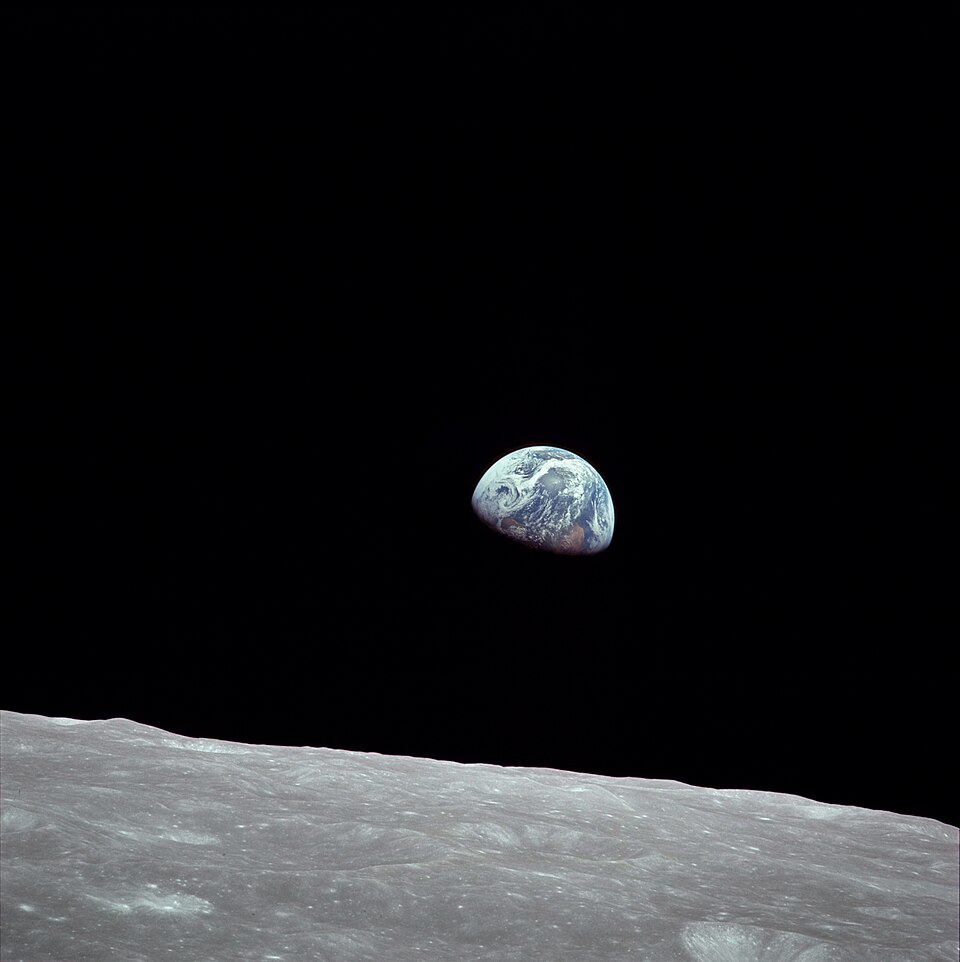
\includegraphics[width=0.85\linewidth]{images/book1/g6-earthrise.jpg}
\end{minipage}\hfill
\begin{minipage}[c]{0.5\linewidth}
{\small \emph{Earthrise} (aardopkomst): de Aarde boven de horizon van de
Maan, gefotografeerd vanuit Apollo~8 in een baan om de Maan,
24~december~1968. (Foto: NASA, Bill Anders.)}

\medskip
{\small Kijk naar de kleuren: het blauw van de \omterm{def:g2:water-on-earth:ocean}{oceanen}, de witte slierten
van de \omterm{def:g4:clouds-rain-snow:cloud}{wolken}, het bruin van het land. Overal eromheen het zwart van de
ruimte; op de voorgrond de dode grijze bodem van de Maan, zonder water en
zonder lucht.}
\end{minipage}
% ledger: nasa:earthrise
\end{omfigure}

Vanuit de ruimte is de Aarde vooral blauw: de \omterm{def:g2:water-on-earth:ocean}{oceaan} bedekt ongeveer zeven
tiende van haar oppervlak. Witte \omterm{def:g4:clouds-rain-snow:cloud}{wolken} van waterdruppeltjes wervelen erboven,
en wit ijs bedekt de \omterm{def:g3:continents-and-oceans:poles}{polen}. Het land is bruin waar het droog is en groen
waar planten groeien. De lucht zelf is niet te zien, maar de \omterm{def:g4:clouds-rain-snow:cloud}{wolken} die erin
zweven, laten zien dat ze er is. Van alle planeten van het zonnestelsel
laat alleen de Aarde deze kleuren samen zien: vloeibaar water, \omterm{def:g4:clouds-rain-snow:cloud}{wolken} en
levende planten.
% ledger: wss:ocean-cover, nasa:apollo17-earth

\begin{history}[Het lichtblauwe stipje]
\begin{minipage}[c]{0.66\linewidth}
Op 14~februari~1990 was de ruimtesonde Voyager~1 ongeveer 6~miljard
kilometer van de Zon, verder weg dan Neptunus. Voordat ze het zonnestelsel
achter zich liet, draaide ze haar camera om en maakte ze een foto van de
Aarde. Op de foto is onze planeet één helder stipje, kleiner dan een
stofkorrel, gevangen in een straal zonlicht. De sterrenkundige Carl Sagan
schreef erover: ``Kijk nog eens naar dat stipje. Dat is hier. Dat is thuis.
Dat zijn wij.''
% ledger: nasa:pale-blue-dot
\end{minipage}\hfill
\begin{minipage}[c]{0.3\linewidth}\centering
\begin{tikzpicture}
  \node[inner sep=0] (img) {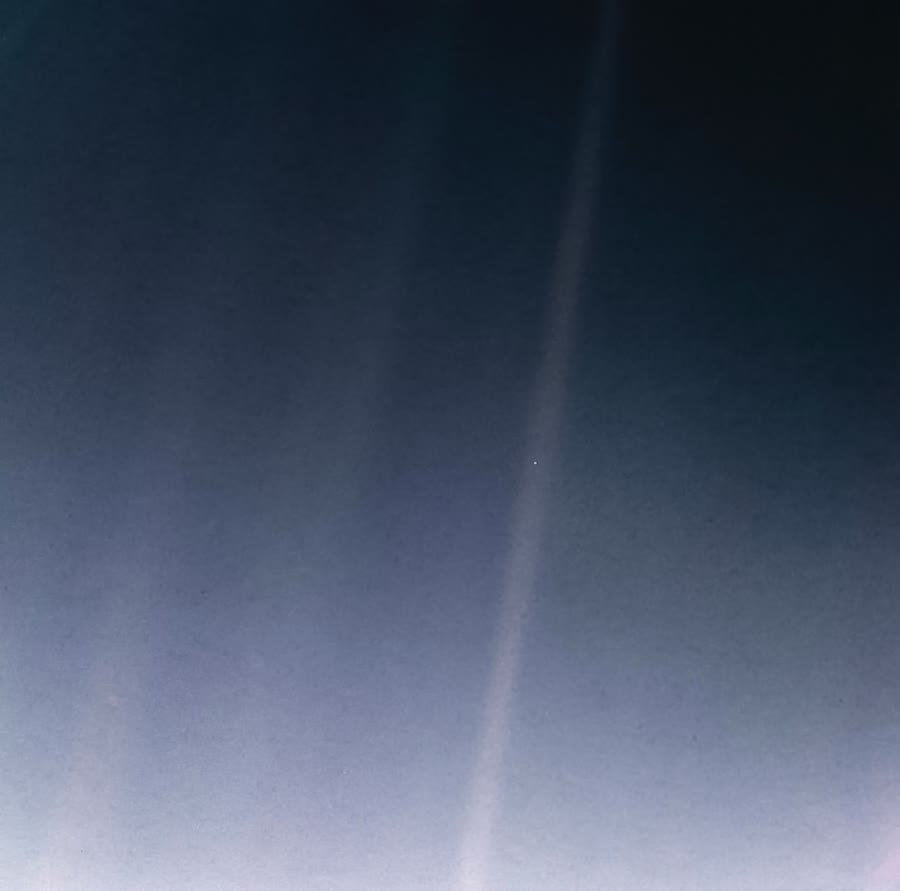
\includegraphics[width=\linewidth]{images/book1/g6-pale-blue-dot.jpg}};
  \draw[yellow!80!orange, thick] ($(img.south west)!0.594!(img.south east) + (0,{0.476*\linewidth})$) circle (6pt);
\end{tikzpicture}\\[2pt]
{\footnotesize De Aarde (omcirkeld) gezien door Voyager~1, 1990. (Beeld:
NASA/JPL-Caltech, publiek domein.)}
% ledger: nasa:pale-blue-dot
\end{minipage}
\end{history}

\section{Oefeningen}

\begin{exercise}[$\star$]\label{exo:g6:earth-a-planet:1}
Noem de acht planeten van het zonnestelsel op volgorde, van de planeet die
het dichtst bij de Zon staat tot de verste. Onderstreep de \omterm{def:g6:earth-a-planet:planet-types}{rotsplaneten}.
\end{exercise}

\begin{exercise}[$\star$]\label{exo:g6:earth-a-planet:2}
Neem over en vul aan: ``Een \omterm{def:g6:earth-a-planet:planet-types}{rotsplaneet} is klein en heeft een grote
\ldots, met een vast \ldots{} Een \omterm{def:g6:earth-a-planet:planet-types}{reuzenplaneet} is heel groot, met een
kleine \ldots, en bestaat vooral uit \ldots{} en \ldots{}''
\end{exercise}

\begin{exercise}[$\star$]\label{exo:g6:earth-a-planet:3}
Welke planeet heeft volgens de tabel van dit hoofdstuk de diameter die het
dichtst bij die van de Aarde ligt? Welke is de grootste planeet? Welke de
kleinste?
\end{exercise}

\begin{exercise}[$\star$]\label{exo:g6:earth-a-planet:4}
Waar of niet waar? Verbeter de zinnen die niet waar zijn.
(a) Venus is bedekt met \omterm{def:g2:water-on-earth:ocean}{oceanen}.
(b) Mars is kouder dan de Aarde.
(c) De \omterm{def:g6:earth-a-planet:planet-types}{reuzenplaneten} zijn de vier planeten die het dichtst bij de Zon staan.
(d) Saturnus heeft een kleinere dichtheid dan water.
\end{exercise}

\begin{exercise}[$\star\star$]\label{exo:g6:earth-a-planet:5}
De diameter van Mercurius is 4\,879~km, de diameter van de Aarde
12\,756~km. Bereken de diameter van Mercurius als percentage van die van de
Aarde, afgerond op een heel getal.
% ledger: planet:Mercury.diameter, planet:Earth.diameter (planets.py: 38.2 %)
\end{exercise}

\begin{exercise}[$\star\star$]\label{exo:g6:earth-a-planet:6}
Hoeveel Aardes naast elkaar passen er in de diameter van Saturnus
(120\,536~km)? Rond af op een heel getal. Is Saturnus een \omterm{def:g6:earth-a-planet:planet-types}{rotsplaneet} of
een \omterm{def:g6:earth-a-planet:planet-types}{reuzenplaneet}?
% ledger: planet:Saturn.diameter, planet:Earth.diameter
\end{exercise}

\begin{exercise}[$\star\star$]\label{exo:g6:earth-a-planet:7}
Sterrenkundigen hebben planeten rond andere sterren gevonden. Planeet~A
heeft een dichtheid van 1.1~gram per kubieke centimeter en is 9~keer zo
breed als de Aarde. Planeet~B heeft een dichtheid van 5.0~gram per kubieke
centimeter en is iets kleiner dan de Aarde. Welke is een \omterm{def:g6:earth-a-planet:planet-types}{rotsplaneet} en
welke een \omterm{def:g6:earth-a-planet:planet-types}{reuzenplaneet}? Leg uit.
\end{exercise}

\begin{exercise}[$\star\star$]\label{exo:g6:earth-a-planet:8}
Gebruik het diagram van de temperaturen van de planeten: (a) hoeveel graden
heter is Venus dan de Aarde? (b) Hoeveel graden kouder is Mars dan de
Aarde?
% ledger: planet:Venus.Tmean, planet:Earth.Tmean, planet:Mars.Tmean
\end{exercise}

\begin{exercise}[$\star\star$]\label{exo:g6:earth-a-planet:9}
Mercurius staat het dichtst bij de Zon, maar Venus is de heetste planeet.
Leg uit waarom.
\end{exercise}

\begin{exercise}[$\star\star$]\label{exo:g6:earth-a-planet:10}
De Aarde staat 150~miljoen kilometer van de Zon en Mars 228~miljoen
kilometer. Hoeveel miljoen kilometer verder van de Zon staat Mars? Hoeveel
procent groter is de afstand van Mars dan die van de Aarde (afgerond op een
heel getal)?
% ledger: planet:Earth.dist, planet:Mars.dist
\end{exercise}

\begin{exercise}[$\star\star\star$]\label{exo:g6:earth-a-planet:11}
Een vriend zegt: ``Mars is altijd een droge \omterm{def:g5:weather-and-climate:desert}{woestijn} geweest; er is daar
nooit water geweest.'' Geef hem met dit hoofdstuk antwoord: wat had Mars
miljarden jaren geleden, waar is zijn water nu, en waarom kan vloeibaar
water nu niet aan zijn oppervlak blijven?
\end{exercise}

\begin{exercise}[$\star\star\star$]\label{exo:g6:earth-a-planet:12}
Venus wordt soms de tweelingzus van de Aarde genoemd. Haar diameter is
95~\% van die van de Aarde, en de zwaartekracht aan haar oppervlak is 8.9
op een schaal waarop die van de Aarde 9.8 is. (a) Bereken de zwaartekracht
op Venus als percentage van die op Aarde, afgerond op een heel getal.
(b) Noem twee manieren waarop Venus op een tweelingzus van de Aarde lijkt,
en twee manieren waarop niet.
% ledger: planet:Venus.gravity, planet:Earth.gravity, planet:Venus.diameter
\end{exercise}

\section{Probleem: Ansichtkaarten van drie planeten}

\begin{problem}[{Weekendprobleem --- drie ansichtkaarten uit de ruimte, en
hoe hard de lucht van Venus op haar grond drukt}]
\label{pb:g6:earth-a-planet:1}
% ledger: planet:Venus.dist, planet:Venus.diameter, planet:Venus.density, planet:Venus.Tmean, planet:Venus.psurf, planet:Earth.dist, planet:Earth.diameter, planet:Earth.density, planet:Earth.Tmean, planet:Earth.psurf, planet:Mars.dist, planet:Mars.diameter, planet:Mars.density, planet:Mars.Tmean, planet:Mars.psurf, nasa:venus-clouds, nasa:mars-water
Drie robotsondes sturen elk een ansichtkaart naar huis, met een paar
getallen op de achterkant.

\begin{center}
\small
\begin{tabular}{>{\raggedright\arraybackslash}p{0.29\linewidth}>{\raggedright\arraybackslash}p{0.29\linewidth}>{\raggedright\arraybackslash}p{0.29\linewidth}}
\hline
\textbf{Van Venus} & \textbf{Van de Aarde} & \textbf{Van Mars}\\
\hline
Afstand tot de Zon: 108~miljoen~km. & Afstand tot de Zon:
150~miljoen~km. & Afstand tot de Zon: 228~miljoen~km.\\
Diameter: 12\,104~km. & Diameter: 12\,756~km. & Diameter: 6\,792~km.\\
Dichtheid: 5.2~g/cm$^3$. & Dichtheid: 5.5~g/cm$^3$. & Dichtheid: 3.9~g/cm$^3$.\\
Gemiddelde temperatuur: 464~$^\circ$C. & Gemiddelde temperatuur: 15~$^\circ$C. &
Gemiddelde temperatuur: $-65$~$^\circ$C.\\
De lucht drukt met 92~bar op de grond. Dikke \omterm{def:g4:clouds-rain-snow:cloud}{wolken} van zuur. &
De lucht drukt met 1~bar op de grond. \omterm{def:g2:water-on-earth:ocean}{Oceanen} en \omterm{def:g4:clouds-rain-snow:cloud}{wolken}. &
De lucht drukt met 0.01~bar op de grond. IJs op de \omterm{def:g3:continents-and-oceans:poles}{polen}.\\
\hline
\end{tabular}
\end{center}

\medskip
\noindent\textbf{Deel I --- De planeten vergeleken.}
\begin{enumerate}
  \item Zet de drie planeten op volgorde van afstand tot de Zon.
  \item Hoeveel miljoen kilometer dichter bij de Zon dan de Aarde staat
        Venus? Hoeveel miljoen kilometer verder staat Mars?
  \item Bereken de diameter van Mars als percentage van die van de Aarde,
        afgerond op een heel getal. Is Mars ongeveer een kwart, de helft of
        drie kwart zo breed als de Aarde?
  \item Zijn de drie planeten \omterm{def:g6:earth-a-planet:planet-types}{rotsplaneten} of \omterm{def:g6:earth-a-planet:planet-types}{reuzenplaneten}? Aan welke
        getallen op de ansichtkaarten zie je dat?
\end{enumerate}

\medskip
\noindent\textbf{Deel II --- De lucht.}
\begin{enumerate}[resume]
  \item Op welke planeet is de lucht het dikst? Op welke het ijlst?
  \item Hoeveel keer minder drukt de lucht van Mars op zijn grond dan de
        lucht van de Aarde op die van ons?
  \item Venus staat dichter bij de Zon dan de Aarde, maar dat alleen
        verklaart geen temperatuur van 464~$^\circ$C. Wat doet de lucht van
        Venus met de warmte van de Zon?
  \item Hoeveel keer zo hard als op Aarde drukt de lucht op de grond van
        Venus? Waarom moet een sonde die op Venus landt heel sterke wanden hebben?
\end{enumerate}

\medskip
\noindent\textbf{Deel III --- Water en leven.}
\begin{enumerate}[resume]
  \item Aan het aardoppervlak bevriest water bij 0~$^\circ$C en kookt het
        bij 100~$^\circ$C. Leg met de gemiddelde temperaturen uit waarom
        water op Aarde vloeibaar is.
  \item Wat zou er gebeuren met een glas water dat op de grond van Venus
        wordt gezet? En op de grond van Mars?
  \item Mars had miljarden jaren geleden \omterm{def:g1:landscapes-around-us:water}{rivieren} en \omterm{def:g1:landscapes-around-us:water}{meren}. Wat zegt dat
        over het \omterm{def:g5:weather-and-climate:climate}{klimaat} van Mars van lang geleden, vergeleken met nu?
  \item Schrijf de achterkant van de ansichtkaart van de Aarde: geef in een
        paar zinnen vier redenen waarom leven op Aarde mogelijk is.
\end{enumerate}
\end{problem}
